\section{改变计算公式}
\label{sec:vr-change-formula}

上一节保持被平均的对象不变，改变样本从哪里来。本节反过来：样本仍按$P$抽取，但不再直接平均$f(X)$，而是平均另一个期望同为$I$、波动更小的量。构造这样的量有两条路。一是找一个与$f$同步起伏、期望已知的辅助量，把可以预测的那部分波动减掉；二是把输入中的一部分随机性用条件平均精确地算掉，只对剩下的部分抽样。两种做法都会增加每个样本的计算，比较时要按第~\ref{sec:vr-comparison}节计入成本。

\subsection{控制变量}
\label{sec:vr-control-variates}

回到导言的第二个例子：
\[
 I=\int_0^1\mathrm{e}^{u}\,\mathrm{d}u=\mathrm{e}-1 .
\]
按$U\sim\operatorname{Unif}(0,1)$抽样，$\mathrm{e}^{U}$的方差为
\[
 \sigma^2=\mathbb{E}\bigl[\mathrm{e}^{2U}\bigr]-(\mathrm{e}-1)^2=\frac{\mathrm{e}^2-1}{2}-(\mathrm{e}-1)^2\approx0.2420 .
\]
这些波动的主要来源一目了然：$U$偏大，$\mathrm{e}^{U}$就偏大。而$U$本身的期望$1/2$是已知的。如果某次抽到的$U$比$1/2$大了$0.1$，就可以预先判断$\mathrm{e}^{U}$大约偏高了$0.1$乘以某个斜率，把这一部分减掉。

\begin{definition}[控制变量估计]
\label{def:vr-control-variate}
设$h$是一个在$P$下期望$\mu_h=\mathbb{E}_P[h(X)]$已知的函数，$\beta$为实数。对独立且都服从$P$的$X_1,\dots,X_n$，称
\begin{equation}
 \hat{I}_n^{\mathrm{CV}}(\beta)=\frac1n\sum_{i=1}^{n}\Bigl[f(X_i)-\beta\bigl(h(X_i)-\mu_h\bigr)\Bigr]
 \label{eq:vr-control-variate}
\end{equation}
为以$h$为\term{控制变量}（control variate）、系数为$\beta$的估计。
\end{definition}

减去的量期望为零，所以对任意固定的$\beta$，估计都无偏。要选的是使方差最小的$\beta$。

\begin{theorem}[控制变量的最优系数]
\label{thm:vr-control-variate}
设$\mathbb{E}_P[f^2]<\infty$，$\mathbb{E}_P[h^2]<\infty$，$\sigma_h^2=\operatorname{Var}_P(h)>0$，记$\sigma_f^2=\operatorname{Var}_P(f)$，$\gamma=\operatorname{Cov}_P(f,h)$。对固定的$\beta$，
\begin{equation}
 n\operatorname{Var}\bigl(\hat{I}_n^{\mathrm{CV}}(\beta)\bigr)=\sigma_f^2-2\beta\gamma+\beta^2\sigma_h^2 .
 \label{eq:vr-cv-variance}
\end{equation}
它在
\begin{equation}
 \beta^{*}=\frac{\gamma}{\sigma_h^2}
 \label{eq:vr-cv-beta}
\end{equation}
处取到最小值$\sigma_f^2(1-\rho^2)$，其中$\rho=\gamma/(\sigma_f\sigma_h)$是$f(X)$与$h(X)$的相关系数（$\sigma_f=0$时最小值为$0$）。
\end{theorem}

\begin{proof}
单项$f-\beta(h-\mu_h)$的方差由方差与协方差的双线性得到$\sigma_f^2-2\beta\gamma+\beta^2\sigma_h^2$，独立平均再除以$n$，这是式~\eqref{eq:vr-cv-variance}。对$\beta$配方：
\[
 \sigma_f^2-2\beta\gamma+\beta^2\sigma_h^2=\sigma_h^2\Bigl(\beta-\frac{\gamma}{\sigma_h^2}\Bigr)^2+\sigma_f^2-\frac{\gamma^2}{\sigma_h^2} .
\]
第一项非负，在$\beta=\beta^{*}$时为零。最小值$\sigma_f^2-\gamma^2/\sigma_h^2$在$\sigma_f>0$时写成$\sigma_f^2(1-\rho^2)$。
\end{proof}

\paragraph{这是一次投影}
把中心化的$f-I$与$h-\mu_h$看成平方可积随机变量空间中的两个向量，$\beta^{*}(h-\mu_h)$正是$f-I$在$h-\mu_h$方向上的正交投影，剩下的$f-I-\beta^{*}(h-\mu_h)$与$h$不相关。也可以说：用$h$对$f$作线性回归，$\beta^{*}$是回归斜率，控制变量估计平均的是回归残差加上$I$。$h$能解释$f$的方差比例为$\rho^2$，这部分被消去，只剩$1-\rho^2$。同时用$k$个控制变量$\bm{h}=(h_1,\dots,h_k)$时，若它们的协方差矩阵$\bm{\Sigma}_{\bm{h}}$可逆，同样配方可得最优系数向量$\bm{\Sigma}_{\bm{h}}^{-1}\operatorname{Cov}_P(\bm{h},f)$，即向$k$维子空间的投影。

\paragraph{例子的数值}
对$f(u)=\mathrm{e}^{u}$与$h(u)=u$，$\mu_h=1/2$，$\sigma_h^2=1/12$。由分部积分，
\[
 \mathbb{E}\bigl[U\mathrm{e}^{U}\bigr]=\int_0^1u\mathrm{e}^{u}\,\mathrm{d}u=\bigl[(u-1)\mathrm{e}^{u}\bigr]_0^1=1 .
\]
于是
\[
 \gamma=1-\frac{\mathrm{e}-1}{2}\approx0.14086,\qquad \beta^{*}=12\gamma\approx1.6903 .
\]
最小方差为
\[
 \sigma_f^2-\frac{\gamma^2}{\sigma_h^2}=0.24204-12\times0.14086^2\approx0.003940 ,
\]
$\rho^2\approx0.984$，方差降为原来的$1/61$。$h(U)=U$在抽样时已经得到，几乎不增加成本，相对效率约为$61$。

图~\ref{fig:vr-control-variate}(a)显示了抵消是怎样发生的：蓝色的$\mathrm{e}^{u}$在$[0,1]$上从$1$升到$2.72$，减去紫色直线$I+\beta^{*}(u-\tfrac12)$的倾斜部分后，绿色的被平均函数只在$1.65$到$1.88$之间变化。剩下的波动来自$\mathrm{e}^{u}$的弯曲，线性的$h$抵消不了它。图(b)是式~\eqref{eq:vr-cv-variance}作为$\beta$的函数：一条开口向上的抛物线，$\beta=0$是直接平均，$\beta^{*}$处取最小。

\begin{BookInlineFigure}
 \centering
 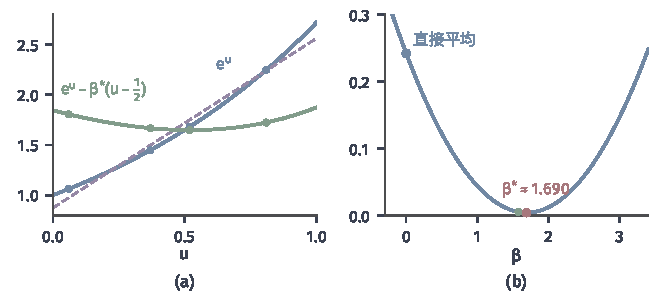
\includegraphics[width=112mm]{figures/07-probability/08-sampling-and-integration/matplotlib/vr-control-variate/figure.pdf}
 \caption{以$h(U)=U$为控制变量计算$\int_0^1\mathrm{e}^{u}\,\mathrm{d}u$。(a)蓝线为$\mathrm{e}^{u}$，紫色虚线为$I+\beta^{*}(u-\tfrac12)$，绿线为$\mathrm{e}^{u}-\beta^{*}(u-\tfrac12)$；圆点标出$u=0.37,0.81,0.06,0.52$处的值。(b)单样本方差$\sigma_f^2-2\beta\gamma+\beta^2/12$随$\beta$的变化：蓝点为直接平均，红点为$\beta^{*}$，绿点为由四个样本估计的$\hat{\beta}=1.577$。}
 \label{fig:vr-control-variate}
\end{BookInlineFigure}

\paragraph{系数由同一批样本估计}
实际中$\gamma$通常未知，$\beta^{*}$也就未知。最直接的办法是用同一批样本的样本协方差与样本方差估计它：
\begin{equation}
 \hat{\beta}=\frac{\sum_{i=1}^{n}\bigl(h(X_i)-\bar{h}\bigr)\bigl(f(X_i)-\bar{f}\bigr)}{\sum_{i=1}^{n}\bigl(h(X_i)-\bar{h}\bigr)^2} ,
 \label{eq:vr-cv-beta-hat}
\end{equation}
其中$\bar{f}$、$\bar{h}$是两列值的样本平均，再代入估计：
\[
 \hat{I}_n^{\mathrm{CV}}(\hat{\beta})=\bar{f}-\hat{\beta}(\bar{h}-\mu_h) .
\]这时减去的量$\hat{\beta}(\bar{h}-\mu_h)$是两个随机量的乘积，它的期望一般不为零：
\[
 \mathbb{E}\bigl[\hat{I}_n^{\mathrm{CV}}(\hat{\beta})\bigr]-I=-\mathbb{E}\bigl[\hat{\beta}(\bar{h}-\mu_h)\bigr]=-\operatorname{Cov}(\hat{\beta},\bar{h}) .
\]
这一偏差通常与$1/n$同阶。

另一方面，
\[
 \hat{I}_n^{\mathrm{CV}}(\hat{\beta})-\hat{I}_n^{\mathrm{CV}}(\beta^{*})=-(\hat{\beta}-\beta^{*})(\bar{h}-\mu_h) ,
\]
两个因子都以$n^{-1/2}$的速度趋于零，乘积是更高阶的量。所以样本量大时，用$\hat{\beta}$与用$\beta^{*}$的渐近方差相同，有限样本则多出一个偏差。

下面用四个均匀随机数逐步演示：
\[
 u=0.37,\quad 0.81,\quad 0.06,\quad 0.52 .
\]
函数值为
\[
 \mathrm{e}^{u}=1.44773,\quad 2.24791,\quad 1.06184,\quad 1.68203 ,
\]
直接平均$\bar{f}=1.60988$，$\bar{h}=0.44$。样本协方差与样本方差（分母都取$3$）分别为$0.15382$与$0.09753$，于是$\hat{\beta}=1.5771$。代入得
\[
 \hat{I}_4^{\mathrm{CV}}(\hat{\beta})=1.60988-1.5771\times(0.44-0.5)=1.70450 .
\]
若用$\beta^{*}$，结果是$1.71130$；真值为$1.71828$。四个样本的$\bar{h}$偏小$0.06$，直接平均随之偏低；控制变量按斜率把这一偏低补了回来。

\paragraph{独立预估系数}
若想保留严格的无偏性，可以用一批与正式样本独立的预备样本估计系数，得到$\widetilde{\beta}$，再在正式计算中当作常数使用。给定$\widetilde{\beta}$，由定义~\ref{def:vr-control-variate}后的论证，条件期望为$I$，所以估计无偏。由全方差公式，它的方差是$\mathbb{E}[\sigma^2(\widetilde{\beta})]/n$，其中$\sigma^2(\beta)$是式~\eqref{eq:vr-cv-variance}的右边；由配方结果，
\[
 \mathbb{E}\bigl[\sigma^2(\widetilde{\beta})\bigr]=\sigma_f^2(1-\rho^2)+\sigma_h^2\,\mathbb{E}\bigl[(\widetilde{\beta}-\beta^{*})^2\bigr] .
\]
最后一项是系数估计不准的代价。预备样本和每个样本上$h$的求值都要计入成本；$h$本身昂贵时，即使$\rho^2$很大，相对效率也可能不高。

\subsection{条件期望降方差}
\label{sec:vr-conditioning}

第~\ref{chap:laws-of-large-numbers}章用随机投点估计过四分之一圆的面积：设$X$与$Y$独立，都服从$\operatorname{Unif}(0,1)$，点落在单位圆内的概率是
\[
 I=\mathbb{P}(X^2+Y^2\leq1)=\frac{\pi}{4} .
\]
直接平均的是示性值$f(X,Y)=\mathbf{1}_{\{X^2+Y^2\leq1\}}$，每个样本只回答“在圆内吗”，单样本方差是$\tfrac{\pi}{4}(1-\tfrac{\pi}{4})\approx0.1685$。可是一旦知道$X=x$，点落在圆内当且仅当$Y\leq\sqrt{1-x^2}$，这件事的概率可以直接写出：
\[
 g(x)=\mathbb{P}\bigl(Y\leq\sqrt{1-x^2}\bigr)=\sqrt{1-x^2} .
\]
那么$Y$就不必再抽了：只抽$X$，平均$g(X)$。

\begin{theorem}[条件期望不增加方差]
\label{thm:vr-conditioning}
设输入为$(X,Y)$，$\mathbb{E}[f(X,Y)^2]<\infty$，记$g(X)=\mathbb{E}[f(X,Y)\mid X]$。则
\begin{equation}
 \mathbb{E}[g(X)]=I,\qquad \operatorname{Var}\bigl(g(X)\bigr)=\operatorname{Var}\bigl(f(X,Y)\bigr)-\mathbb{E}\bigl[\operatorname{Var}\bigl(f(X,Y)\bigm|X\bigr)\bigr] .
 \label{eq:vr-conditioning}
\end{equation}
所以对独立且同分布的$X_1,\dots,X_n$，平均$g(X_i)$的方差不超过同样个数的独立$(X_i,Y_i)$上平均$f$的方差；等号当且仅当$\operatorname{Var}(f(X,Y)\mid X)=0$几乎必然成立。
\end{theorem}

\begin{proof}
第一式是全期望公式。第二式是第~\ref{chap:conditional-expectation}章的全方差公式移项：
\[
 \operatorname{Var}(f)=\mathbb{E}\bigl[\operatorname{Var}(f\mid X)\bigr]+\operatorname{Var}\bigl(\mathbb{E}[f\mid X]\bigr) .
\]
减去的一项非负，所以$\operatorname{Var}(g(X))\leq\operatorname{Var}(f)$。两种平均都是$n$个独立同分布项的平均，方差各除以$n$，大小关系保持。减去的项为零当且仅当条件方差几乎必然为零。
\end{proof}

这种做法称为\term{条件Monte Carlo}（conditional Monte Carlo）。按第~\ref{chap:conditional-expectation}章的说法，条件期望是按$X$分组后的组内平均：直接抽样时，每个样本在自己的组里随机取一个值；条件化以后，每个样本直接报出组内平均。全方差公式中被减去的$\mathbb{E}[\operatorname{Var}(f\mid X)]$正是组内的平均波动，它被精确地算掉了。

\paragraph{四分之一圆的数值}
条件化后的方差为
\[
 \operatorname{Var}\bigl(g(X)\bigr)=\mathbb{E}[1-X^2]-\Bigl(\frac{\pi}{4}\Bigr)^2=\frac23-\frac{\pi^2}{16}\approx0.04982 ,
\]
被消去的组内波动为$0.1685-0.0498=0.1187$，方差降为原来的$1/3.38$。用下面四个点逐步演示：
\[
 (x,y)=(0.37,0.23),\quad(0.81,0.68),\quad(0.06,0.45),\quad(0.52,0.91) .
\]
第二、四个点在圆外，直接平均给出$0.5$，对应$\pi\approx2.0$。条件化只用四个$x$，
\[
 g(x)=0.92903,\quad 0.58643,\quad 0.99820,\quad 0.85417 ,
\]
平均为$0.84196$，对应$\pi\approx3.37$。

\begin{BookInlineFigure}
 \centering
 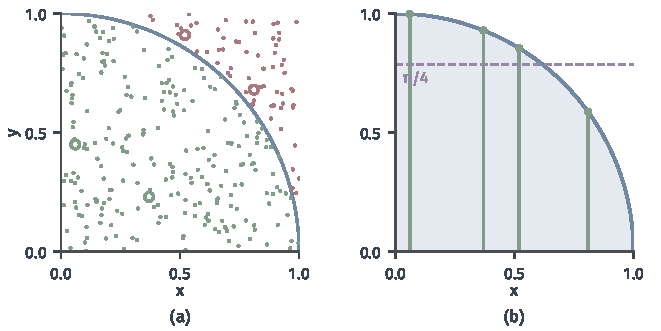
\includegraphics[width=112mm]{figures/07-probability/08-sampling-and-integration/matplotlib/vr-conditional/figure.pdf}
 \caption{用条件期望计算$\mathbb{P}(X^2+Y^2\leq1)=\pi/4$。(a)单位正方形中的$300$个随机点（种子2），圆内为绿色、圆外为红色，四个空心圆为正文的手算点；蓝线是四分之一圆周。(b)蓝线为$g(x)=\sqrt{1-x^2}$，绿色竖线是四个手算点的$x$处整条竖直切片在圆内的比例，紫色虚线为$\pi/4$。}
 \label{fig:vr-conditional}
\end{BookInlineFigure}

图~\ref{fig:vr-conditional}对比了两种计算。左图每个点只给出$0$或$1$；右图每个$x$给出整条竖直切片落在圆内的比例，样本之间的差别只来自$x$的不同。这里$g$只需一次开方，每个样本还少抽一个均匀数，成本不增反减。一般情形下，计算$g$可能需要一个积分，它的成本必须计入。

\paragraph{条件平均只能近似时}
若$g$没有闭式，需要用数值方法近似，定理~\ref{thm:vr-conditioning}的保证不能直接沿用，要看近似怎样做。

一种做法是确定性的求积。例如在每个$x$处，用$m$个等距中点$y_j=(j-\tfrac12)/m$数出满足$x^2+y_j^2\leq1$的比例，作为$g(x)$的近似$g_m(x)$。这个量不是$f$的条件期望，$\mathbb{E}[g_m(X)]\neq I$，产生一个不随$n$减小的偏差，需要像数值积分那样单独估计它的大小。

另一种做法是在每个$X_i$处再独立抽$m$个$Y_{i,1},\dots,Y_{i,m}$，平均$f(X_i,Y_{i,j})$。给定$X_i$时这$m$项独立同分布，所以内层平均的条件期望仍是$g(X_i)$，估计无偏。由全方差公式，内层平均的方差为
\[
 \operatorname{Var}\bigl(g(X)\bigr)+\frac{\mathbb{E}\bigl[\operatorname{Var}(f\mid X)\bigr]}{m} .
\]
$m=1$时回到直接平均，$m\to\infty$时趋于条件Monte Carlo，代价是每个外层样本做$m$次内层计算。四分之一圆中取$m=2$，方差为$0.0498+0.1187/2\approx0.1092$。
